\chapter{Example Application}

In this chapter I will showcase the development of an example project that aims to demonstrate the capabilities of the selected multicore microcontroller and the Rust programming language. I will highlight features that are plain better from most perspectives, as well as the areas where this approach falls short compared to a traditional C project. The example project will have a definite function but the usage of certain peripherals and language features are more in focus thus the functionality may seem a bit purposeless as a real application.

\section{General Description}

The example application implements a very basic webserver on the M7 core of the microcontroller, and does some light signal processing on the M4 core. The general direction of this project was to design one part of the application to use the ethernet peripheral in some capacity, and the other to be capable of doing a task in real time. Also I had to make sure that safe, two-way communication between the two cores is displayed in the application.

Finally an application draft was drawn up. In it the M7 core handles the ethernet peripheral and takes on the role of a simple webserver. It hosts a simple website on a fixed IP address where coefficients of a low pass filter can be supplied. The site also displays the average value of an ADC peripheral. The other core handles the previous ADC peripheral by performs filtering with the coefficients supplied on the website and a fix formula. The filtered signal is emitted on a DAC peripheral with minimal latency latency. An average value is also calculated by the M4 core periodically from a configurable number of samples, this value will be displayed on the website.

\begin{figure}[!ht]
    \centering
    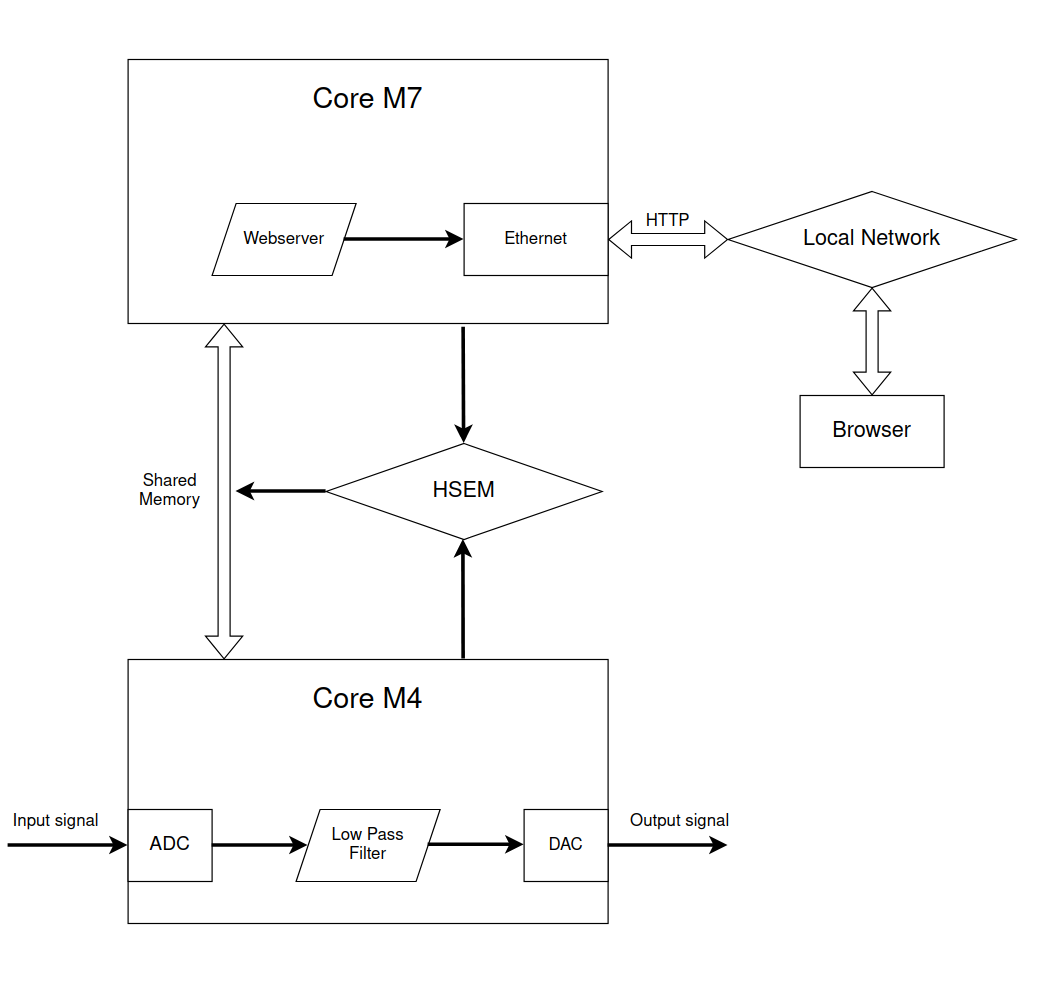
\includegraphics[width=150mm, keepaspectratio]{figures/example-app-flowchart.png}
    \caption{Block Diagram of the Example Application}
    \label{fig:hsem-interrupt-sd}
\end{figure}

With this flow, the application demonstrates the usage of  a decent number of peripherals, namely an ADC, a DAC, ethernet, UART and LEDs for debugging, and of course the hardware semaphores for preventing concurrent shared memory access.

\section{Peripherals}


\subsection{Basic peripherals}

\subsection{Ethernet}

\subsubsection{Driver}
\subsubsection{Smoltcp}
\subsubsection{Connection to TCP stack}

\subsection{ADC}

\subsection{DAC}


\section{Setup Phase}


\section{Main Loop}

\subsection{Webserver}

\subsection{Signal Filtering}
